\section{Evaluation}

\subsection{Efficiency Requirements}\label{eval-efficiency}

In this section, in the view of the memory-computation-energy efficiency requirements, we compare the three baseline algorithms (i.e., model compression, off-the-shelf architecture, and quantization).
%We then select an efficient design scheme for NNs that satisfies all our requirements.


\noindent\textbf{Memory Efficiency.} Off the shelf models are designed to specifically reduce the memory footprint.
For instance, the memory footprint of Squeezenet and MobileNet is 5MB and 14Mb compared to 250Mb of Alexnet and $>$500Mb of VGG architectures~\cite{DBLP:journals/corr/IandolaMAHDK16,conf/cvpr/SandlerHZZC18}.
Additionally, lowering the model precision from 64 or 32 bit floating point to binary precision results in a direct reduction of 64x or 32x in the overall memory footprint of the model.
However, in case of model compression the model parameters which are pruned are simply replaced by a value of "0"  and does not necessarily decrease the overall memory footprint unless the hardware is optimized to skip the storage of all the zero values.


\noindent\textbf{Computation Efficiency.} Design of efficient off-the-shelf architectures replaces the complex matrix-vector multiplications to smaller dimensions.
This reduces the overall number of parameters but it has been shown empirically\footnote{https://github.com/albanie/convnet-burden} that this does not necessarily reduce the number of multiply accumulate operations~\cite{article}.
In case of parameter pruning, achieving efficiency requires additional hardware optimization. Particularly, instead of actually computing the multiplications with "0" pruned values, the hardware optimization enables the user to skip the computation and replace the output by a "0" directly.
For quantized models with binarized parameters and activations the MACs can be replaced by binary XNOR operations, maxpool replaced by OR operation, while the activations can be replaced by checking the sign bit and hence reducing the FLOPS drastically~\cite{235489}.
This results in high computational efficiency and hence, faster inference.



\noindent\textbf{Energy Efficiency.} Energy efficiency does not vary much with reduction of number of parameters and data type, but the number of memory accesses play vital role~\cite{6757323}.
Specifically, for the case of off-the-shelf architectures, while computation efficiency improves, the energy efficiency is close to large scale state of the art models like AlexNet~\cite{DBLP:journals/corr/IandolaMAHDK16,8114708}.
Alternatively, for the case of model compression, energy efficiency can be marginally improved by additionally providing hardware optimization~\cite{journals/corr/YangCS16a,DBLP:journals/corr/HanMD15}.
For quantization, however, the energy efficiency is high as the memory access can be drastically reduced by increasing the throughput of data fetched from the memory.
Specifically, lowering the precision from 32 bit floating point to binary results in lowering the memory accesses and 32x improvement in energy consumption~\cite{NIPS2016_6573,rastegari2016xnornet}.
The benchmarking of energy consumption for different optimization and architectures is well explored and out of scope of this work. We refer the readers to~\cite{8114708} for more details. %in the literature

\textbf{In summary, compared to different optimization techniques, the quantized architectures show significant benefits for different efficiency requirements over the other alternatives.}






\subsection{Privacy Leakage}\label{eval-leakage}

\begin{figure*}[!htb]
    \centering
\subfloat[Impact of Model Pruning on Privacy (FashionMNIST)]{\label{fig:prune}{
  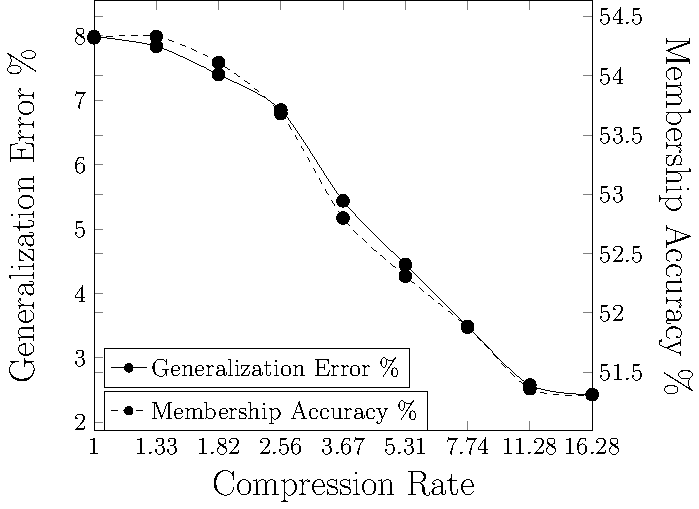
\includegraphics[width=0.28\linewidth]{figures/fmnist_prune.pdf}}}
\hspace{4mm}
\subfloat[Impact of Retraining on Privacy]{\label{fig:retrain}{
  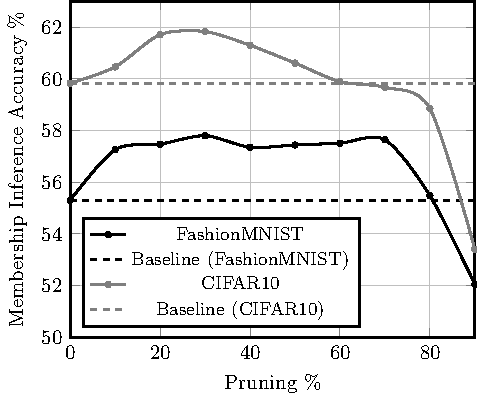
\includegraphics[width=0.28\linewidth]{figures/retrain.pdf}}}
\hspace{4mm}
\subfloat[Mitigating Privacy Leakage via Weight Sharing (FashionMNIST)]{\label{fig:wtsharing}{
  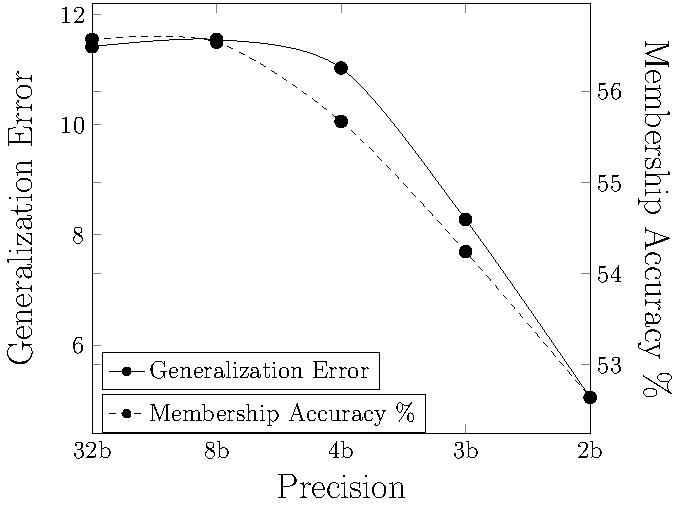
\includegraphics[width=0.28\linewidth]{figures/fmnist_wtsharing.pdf}}}
\vspace{-1mm}
    \caption{Pruning the model lowers the membership inference leakage at the cost of accuracy. Retraining the pruned model to restore accuracy results in a higher membership privacy leakage compared to uncompressed baseline model. This additional leakage can be mitigated by weight sharing at the cost of accuracy.}
    \label{fig:NIAcause}
\end{figure*}

In this section, we evaluate the information leakage through membership inference attacks for the three baseline algorithms considered.

\subsubsection{Model Compression}

We evaluate the privacy leakage on compressing a model by pruning the connections in the model for FashionMNIST and CIFAR10.
As described in the original paper~\cite{Han:2015:LBW:2969239.2969366,DBLP:journals/corr/HanPNMTECTD16}, pruning is followed by retraining the model to restore the model's original accuracy with the pruned connections.

On pruning the model, the model's test accuracy decreases but also lowers the membership inference accuracy. % for FashionMNIST
As the compression rate increases, the generalization error decreases (owing to a decrease in both train and test accuracy) with a decrease in membership accuracy to close to random guess.
This is expected as the parameters are responsible for memorizing the training data information~\cite{DBLP:journals/corr/abs-1812-00910,236216,10.1145/3133956.3134077}. % and pruning the parameters lowers the adversary's attack success.
Interestingly, on retraining the pruned model, we observe that the membership inference accuracy is much higher than the original unpruned baseline model.
This indicates that model compression in turn increases the overall privacy leakage.
This can be attributed to the lower number of parameters forced to learn the same amount of information stored previously in the unpruned model with larger number of parameters (higher memorization of information per parameter).

\textbf{In summary, model compression results in a higher membership privacy leakage compared to the baseline uncompressed model making it a poor candidate for applications with sensitive data.}






\subsubsection{Off-the-Shelf Efficient Architectures}


\begin{table}[h]
\begin{center}
\renewcommand\arraystretch{1.5}
\fontsize{6.5pt}{6.5pt}\selectfont
\begin{tabular}{|c|c|c|c|c|}
\hline
\multicolumn{5}{|c|}{\textbf{CIFAR10}}\\
\hline
\textbf{Architecture} & \textbf{Memory} & \textbf{Train}  & \textbf{Test}  & \textbf{Inference}   \\
 & \textbf{Footprint} & \textbf{Accuracy} & \textbf{Accuracy} & \textbf{Accuracy}  \\
\hline
SqueezeNet & 5 MB & 88.21\% & 81.92\% & \cellcolor{green!25}53.07\% \\
MobileNetV2 & 14 MB & 97.50\% & 87.24\% & \cellcolor{green!25}55.57\% \\
\hline
AlexNet & 240 MB & 97.86\% & 80.34\% & \cellcolor{red!25}60.40\% \\
VGG11 & 507 MB & 99.13\% & 86.43\% & \cellcolor{red!25}58.04\% \\
VGG16 & 528 MB & 99.58\% & 88.95\% & \cellcolor{red!25}58.70\%  \\
VGG19 & 549 MB & 99.09\% & 88.18\% & \cellcolor{red!25}57.85\% \\
\hline
\end{tabular}
\end{center}
\caption{Model complexity influences the membership inference leakage.}
\label{stdarch}
\vspace{-0mm}
\end{table}

In this section, we evaluate two popular state of the art architectures, SqueezeNet and MobileNet, trained on CIFAR10 dataset used for low powered systems.
This evaluation is done only on CIFAR10 dataset as these state of the art architectures are not adapted for the FashionMNIST dataset.
As seen in Table 1, the \textbf{SqueezeNet and MobileNet models shows lower membership inference accuracy of 53.07\% and 55.57\% compared to larger models which have higher privacy leakage (however have poor efficiency compared to alternatives)}.




\subsubsection{Quantization}\label{quant}

We evaluate the technique of reducing the precision of both model's parameters and intermediate activations.
We consider the extreme case of binarizing the parameters and activations allowing to evaluate on the most optimized case.
We evaluate on FashionMNIST dataset for two architectures with convolutional and fully connected layers and CIFAR10 dataset with state of the art architectures.
On replacing the MAC operations with XNOR operations, we observe that the inference risk decreases close to random guess, however, at the cost of prediction test accuracy.

\begin{table}[h]
\begin{center}
\renewcommand\arraystretch{1.5}
\fontsize{6.5pt}{6.5pt}\selectfont
\begin{tabular}{ll}
\begin{tabular}{|c|c|c|c|c|}
\hline
\multicolumn{5}{|c|}{\textbf{FashionMNIST}}\\
\hline
\textbf{Architecture} & \textbf{Memory} & \textbf{Train}  & \textbf{Test}  & \textbf{Inference}  \\
 & \textbf{Accuracy} &  \textbf{Footprint} & \textbf{Accuracy} & \textbf{Accuracy}  \\
\hline
\multicolumn{5}{|c|}{Fully Connected Architecture}\\
Full & 38.39 MB & 100\% & 92.35\% & \cellcolor{red!25}57.46\%\\
XNOR-Net & 1.62 MB & 87.19\% & 85.68\% & \cellcolor{green!25}51.05\%\\ %1,626,824 parameters
\hline
\multicolumn{5}{|c|}{LeNet Architecture}\\
Full & 29.83 MB & 99.34\% & 89.88\% & \cellcolor{red!25}54.86\% \\
XNOR-Net & 0.93 MB & 92.67\% & 86.68\% & \cellcolor{green!25}51.74\%\\ %937,000parameters
\hline
\end{tabular}
&
\begin{tabular}{|c|c|c|c|c|}
\hline
\multicolumn{5}{|c|}{\textbf{CIFAR10}} \\
\hline
\multicolumn{2}{|c|}{\textbf{Architecture}} & \textbf{Train}  & \textbf{Test}  & \textbf{Inference}  \\
 \multicolumn{2}{|c|}{} & \textbf{Accuracy} & \textbf{Accuracy} & \textbf{Accuracy}  \\
\hline
\multirow{2}{*}{NiN} & Full & 98.16\% & 86.16\% & \cellcolor{red!25}56.69\% \\
& XNOR-Net & 81.93\% & 78.74\% & \cellcolor{green!25}51.76\% \\
\hline
\multirow{2}{*}{AlexNet} & Full & 97.86\% & 80.34\% & \cellcolor{red!25}60.40\% \\
& XNOR-Net & 68.62\% & 66.8\% & \cellcolor{green!25}51.40\% \\
\hline
\multirow{2}{*}{VGG13} & Full & 99.58\% & 88.95\% & \cellcolor{red!25}58.70\%\\
& XNOR-Net & 79.67\% & 74.64\% & \cellcolor{green!25}52.65\%\\
\hline
\end{tabular}
\end{tabular}
\end{center}
\caption{Quantized models minimize privacy leakage compared to full precision models due to lower model capacity and hence lower memorization.}
\end{table}


\textbf{In summary, we observe that quantization, specifically binarization of parameters and activation along with XNOR computation, provides strong resistance against inference attacks compared to model compression and off-the-shelf architectures.}
